% !TEX root =  thesis.tex
\chapter{General System Requirements}\label{systemRequirements}

The MASS is designed as a domain independent central process where all domain knowledge is obtained from the SFI and CFI. To prevent any interference or assumption, the MASS and the Agents run as separate independent processes. The cTAEMS model supplies the internal knowledge used to built a Task Tree from which Agents will select available Events for execution. This coupled with the easy configuration mechanism, logging, reporting and statistical analysis makes the simulator a good platform for research and evaluation of Multi-Agent Systems.

\section{System Features}

The following list offers a brief outline and description of the main features and functionalities of the MASS. The features are split into two major categories: core features and optional features. Core features are essential to the application's operation, whereas optional features are preferred but not required. For a better understanding of the basic features of the system see Figure 3.1.
%~\ref{fig:ERD}

\begin{figure}[htb]
\centering
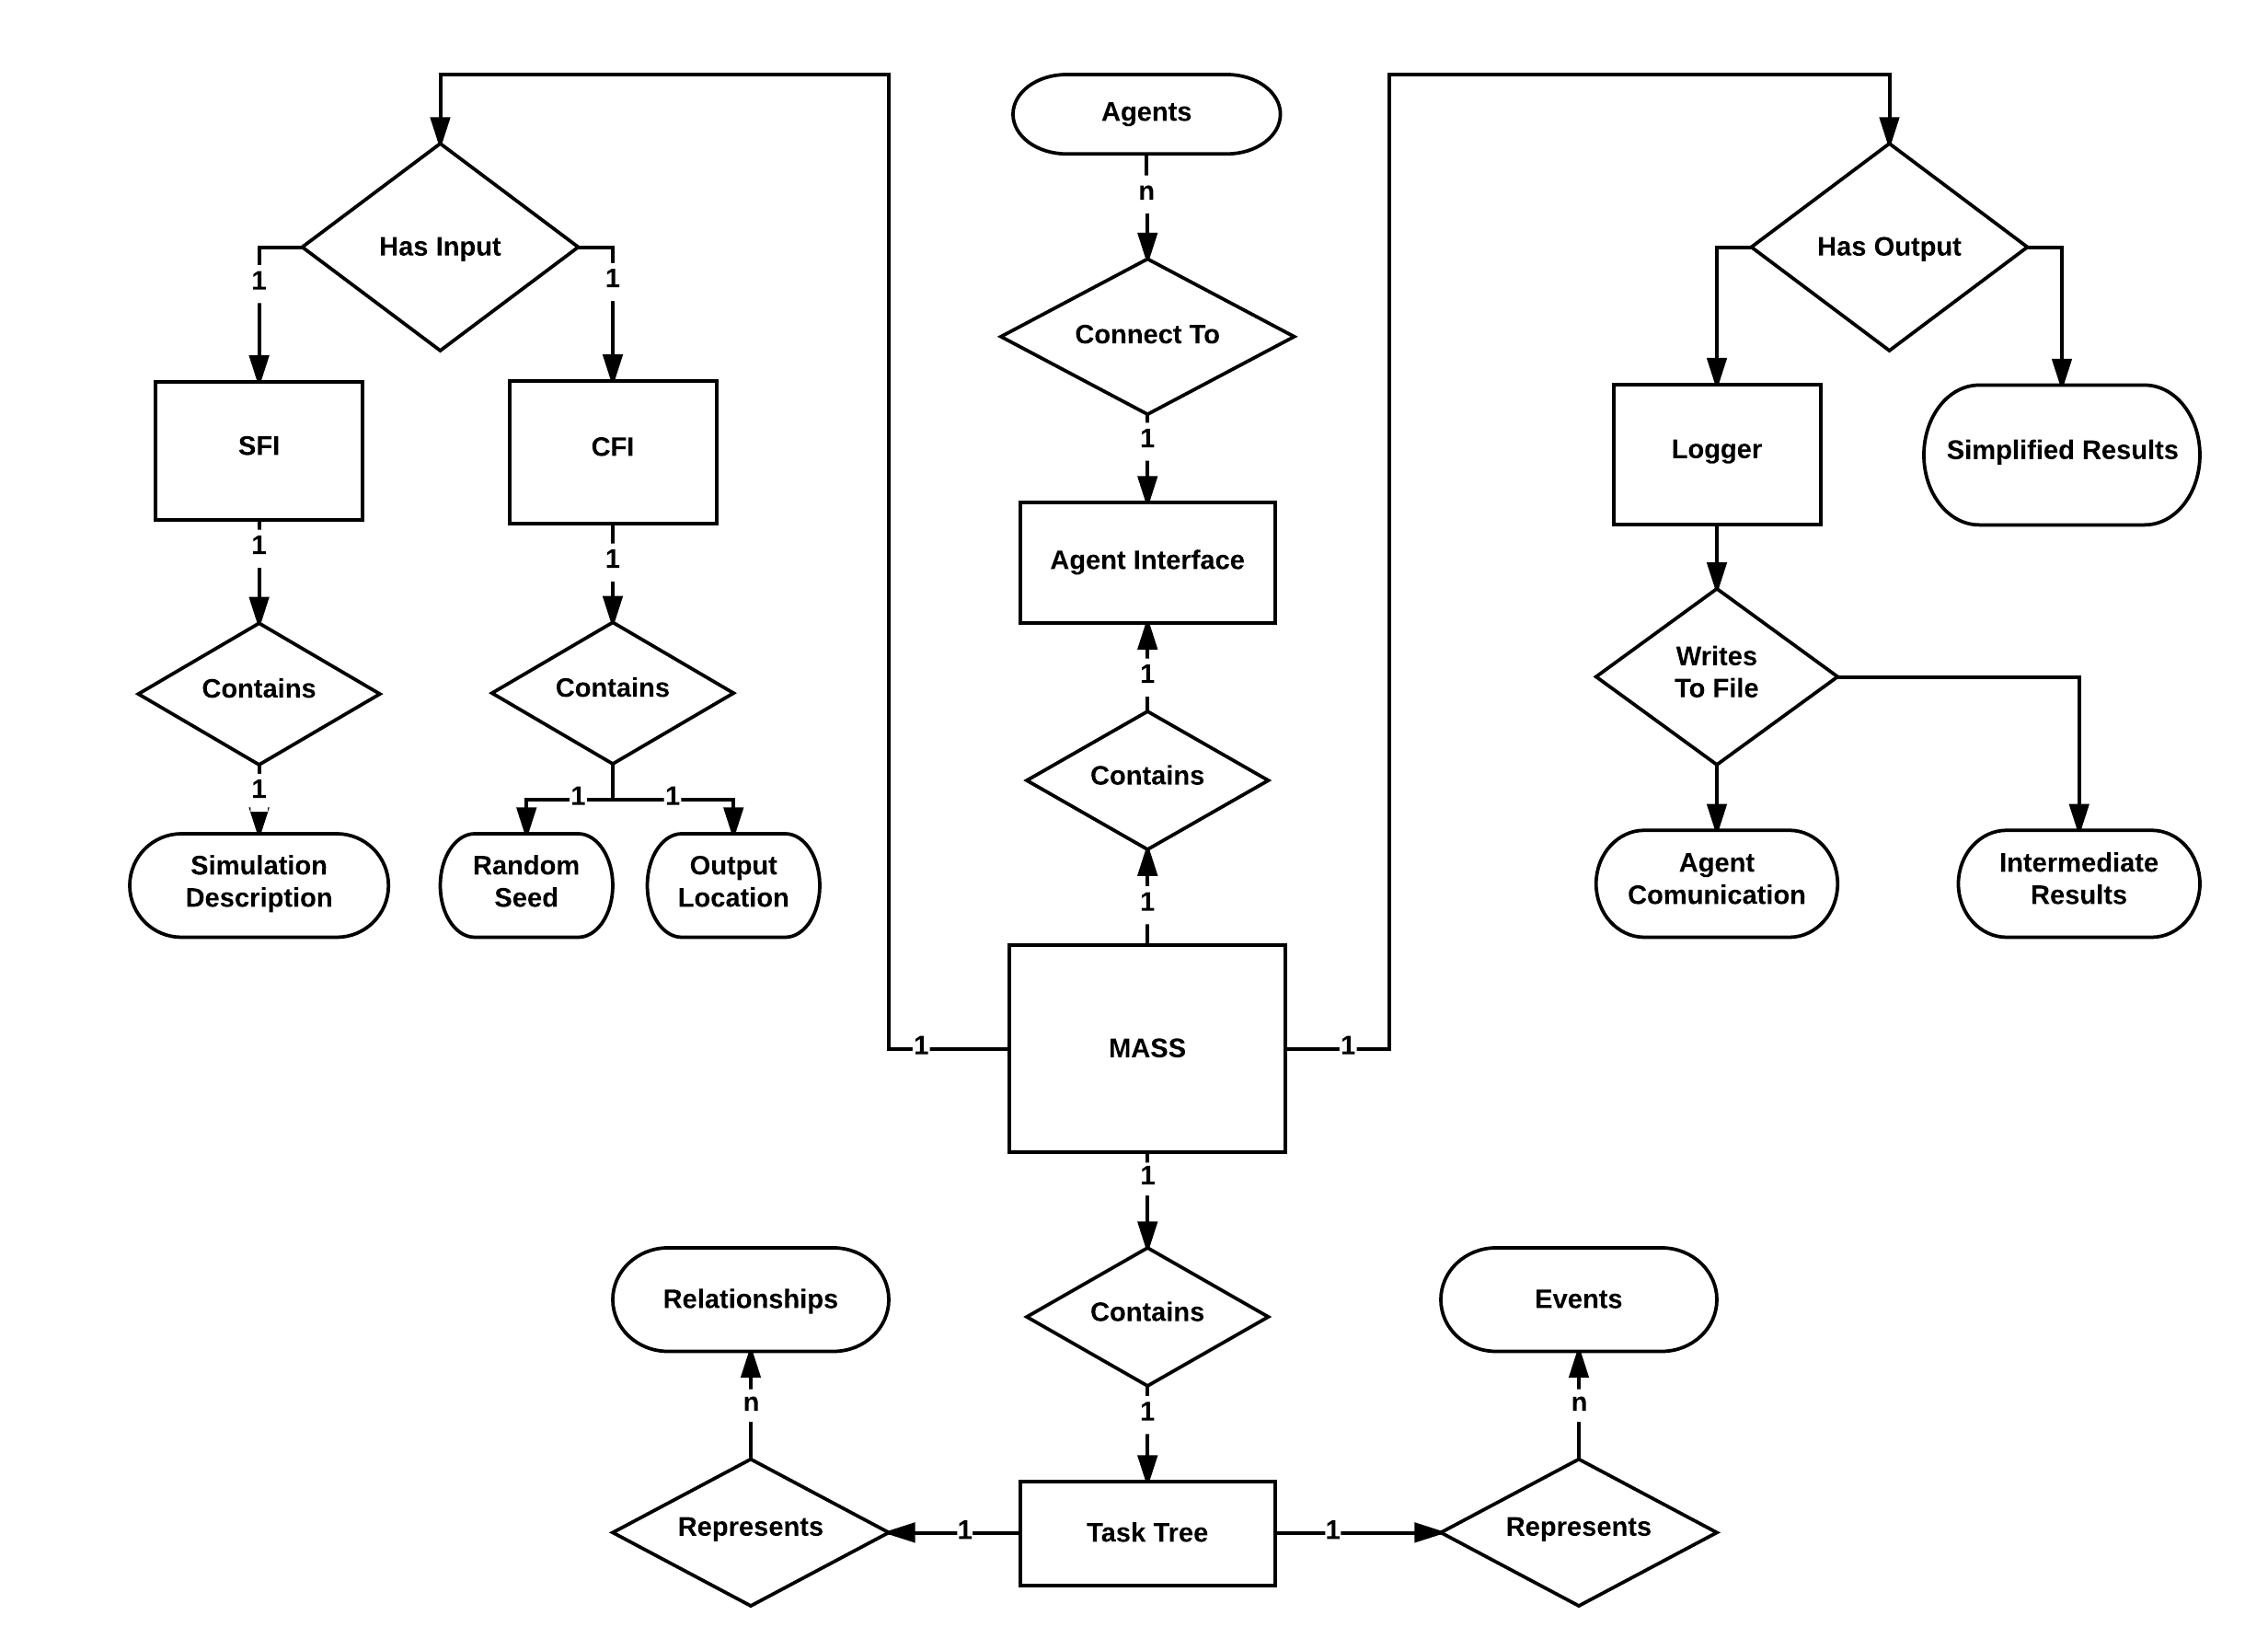
\includegraphics[width=6.5in]{figs/ERD}
\caption{ERD diagram for basic components of MASS.}
\label{fig:ERD }
\end{figure}

\begin{center} \textbf{Core Features} \end{center}


\begin{enumerate}

  \item\textbf{Running The MASS}: The MASS will run via the command line inside of a BASH script that takes as inputs the SFI and optionally the CFI.
  
  \item\textbf{Simulation File Input (SFI)}: The SFI is a cTAEMS file.
    \begin{enumerate}
    \item The system is only required to support the use of the AND, OR, and SUM logical functions of the CTAEMS grammar.
  \end{enumerate}
  
  \item \textbf{Configuration File Input (CFI)}: The program by default will look for a plain text configuration file in the current directory. Optionally, a user can specify the location of this CFI.
  \begin{enumerate}
    \item If no configuration file is found the system will make one in the current directory with default values.
    \item The CFI will contain a random number seed and output file destination.
  \end{enumerate}
  
  \item\textbf{Agent Facing Interface}: The system will provide a consistent interface of which all Agents must implement in order to connect to the internal communication model.
  \begin{enumerate}
    \item All communication between the Agents and the MASS will be represented in the JSON format.
    \item The system must handle any Agent architecture in compliance with the Agent Interface and Simulation structure and refuse connection to any Agent in violation of these elements.
    \end{enumerate}
    
    \item\textbf{Agent Communication}: Agents Must have the ability to communicate throughout the Simulation.
    \begin{enumerate}
    \item An Agent can send a message directly to another Agent.
    \item An Agent can broadcast a message to multiple Agents without explicitly knowing the number of Agents that will receive the message.
  \end{enumerate}
  
  \item\textbf{Simulation Structure}: A Simulation will consist of a Task Tree that keeps track of what Events are able to be executed at any given time.
   \begin{enumerate}
    \item It is the job of the agent to choose from the available Events and report to the Simulation when starting or finishing an event.
  \end{enumerate}
  
  \item\textbf{Creating a Simulation}: A Simulation must be repeatable.
   \begin{enumerate}
    \item Any probability distributions must be computed using the seed value obtained from the CFI before the Simulation begins.
    \item The Task Tree must be built prior to the Simulation?s start.
    \item The MASS must determine what Events within the Task Tree have no dependencies and pass this information to the Agents prior to the Simulation?s start. 
  \end{enumerate}
  
  \item\textbf{Running a Simulation}: The MASS must keep track of Events.
    \begin{enumerate}
    \item The Mass must know what events are able to be executed at any given time.
    \item The Mass must know what events are being executed at any given time.
    \item The Mass must know what events have been executed at any given time.
  \end{enumerate}
  
  \item\textbf{Simulation Output}: The system will produce a command line output detailing the overall Quality, Cost and Duration of the entire Simulation.
  \begin{enumerate}
  \item This output should be clear and concise.
  \end{enumerate}
  
  \item\textbf{Log File Output (LFO)}: The system will produce a detailed log file including the intermediate Quality and Cost between every Task, Subtask, and Method.
  \begin{enumerate}
  \item The LFO will contain a transcript of Agent communication
  \item The LFO will contain compiled statistics on Agent communication frequency.
  \item The LFO will contain the intermediate and final Quality, Cost, and Duration that results from completing an Event in the Task Tree.
  \end{enumerate}

\end{enumerate}


\begin{center} \textbf{Additional Features} \end{center}

\begin{enumerate}

\item\textbf{Graphical Representation of Task Tree}:  The Task Tree is a hierarchical tree-like structure representing Events and the relationship between them.
\begin{enumerate}
\item The system may represent this structure as a graphical model to help understand the Simulation results better. 
\end{enumerate}

\item\textbf{CTAEMS Grammar Support}: The system may go beyond the logical AND, OR, and SUM operations and include additional implementations within the cTAEMS grammar. Figure 3.2 represents a code snippet of CTAMES grammar.

\begin{figure}[htb]
\centering
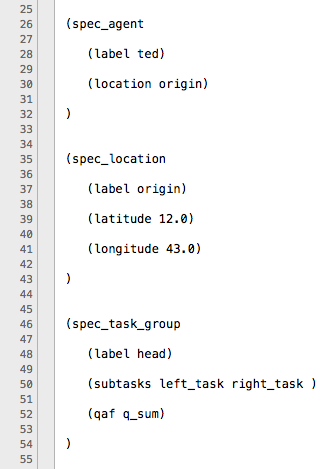
\includegraphics[width=2.0in]{figs/cTAEMS}
\caption{CTAMES grammar}
\label{fig:cTaems }
\end{figure}

\item\textbf{Agent Behavior}: The System may support the ability of Agents to stop, pause, or resume Tasks, Subtasks, and Methods if such actions are applicable based on the Simulation specifications. 

\end{enumerate}
